\section{Implementation}\label{sec:implemenation}

For the implementation we decided to create a multiview application, consisting of 4 views.
The first view shows a parallel coordinate plot.
We decided to use this technique because we want to show more than 2 attributes.
We want to show a user selected consumer and restaurant attribute plus the rating of that consumer for the specific restaurant.
We could also use colors for the rating, but most attributes in the data set only have a few possible values, so there is a lot of overlap.
The result of this overlap is that not all colors are visible.
A parallel coordinate plot also shows dense regions better than other discussed techniques.
The parallel coordinate plot allows the user to select a region on the axis to filter data.
We also add two selection boxes, with these boxes the left and right axis of the parallel coordinate plot can be changed.
The parallel coordinate plot will have three axis, the left axis shows restaurant attributes, the middle the rating and the right axis shows a consumer attribute.
Each line in the parallel coordinate plot represents a consumer restaurant rating.
With the added selection boxes different attributes of the restaurant and consumer can be compared.

The second view is a map with all restaurants, users and their relation.
Each line in the parallel coordinate plot contains a restaurant and a consumer, these are shown as individual markers on the map.
Restaurants and consumer markers have different icons and colors, so they can easily be distinguished by the user.
When a filter is applied in the parallel coordinate plot it is also applied on the map, so geo-location patterns can be investigated.
When a consumer or restaurant marker is selected on the map it is drawn orange, so it can easily be found.
Red lines are drawn from the selected marker, these represent ratings.
These ratings are also highlighted in the parallel coordinate plot, as shown in the top views of figure~\ref{dashboard-view}.
In this figure a filter is applied on the middle axis of the parallel coordinate plot.

\begin{figure}[h!]
 \centering
 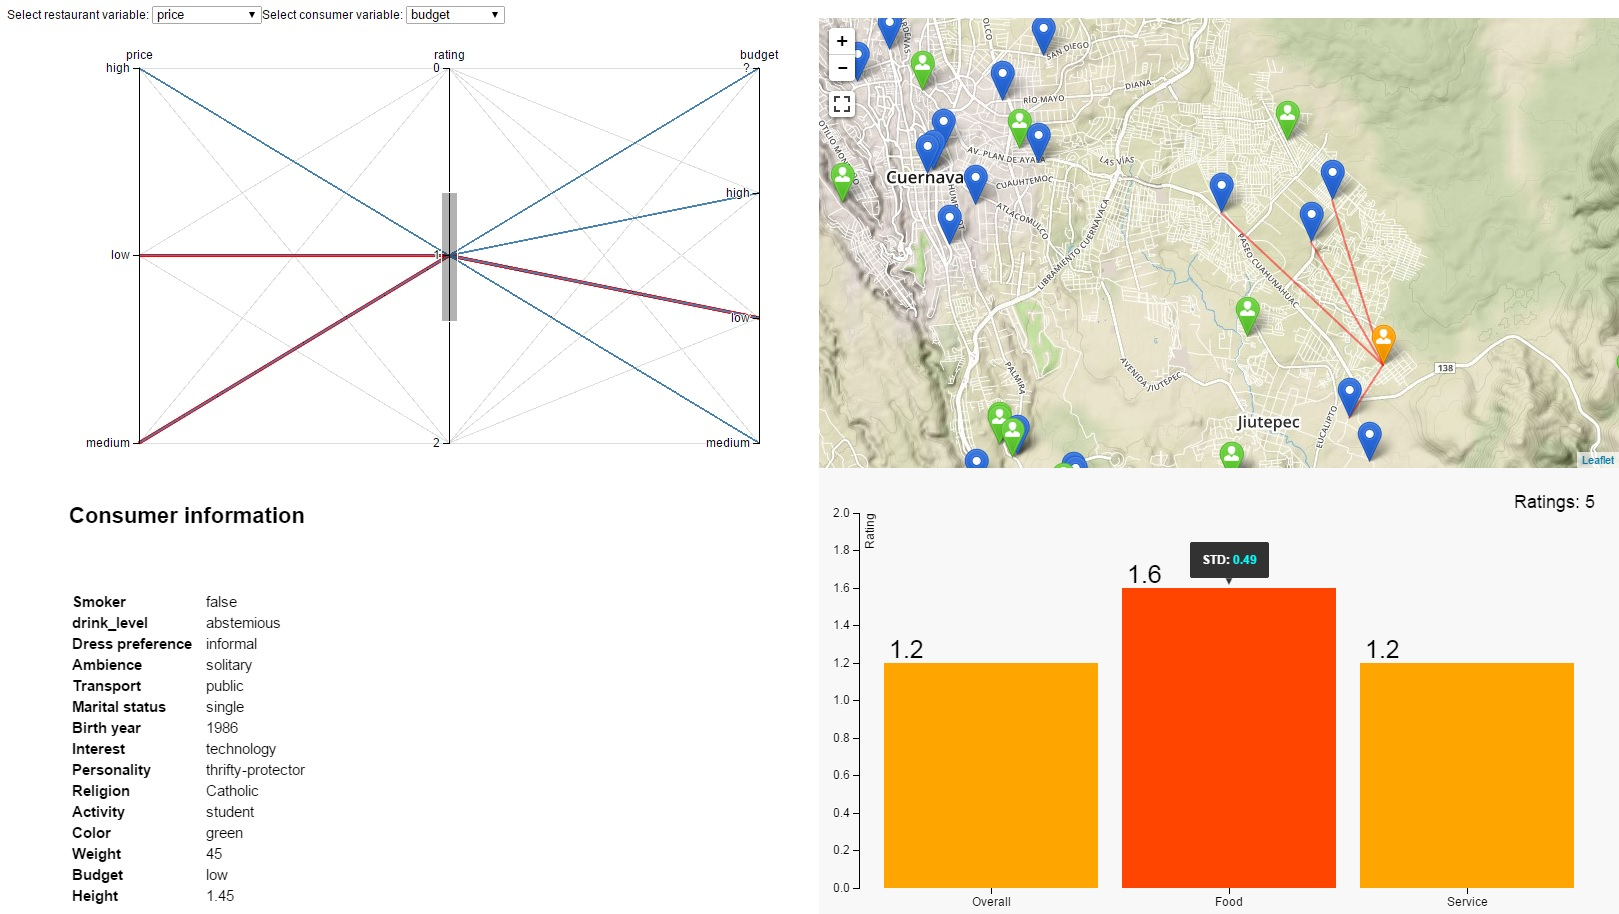
\includegraphics[width=1\textwidth]{img/dashboard-final.jpg}
 \caption{Final multiview dashboard visualization.}
 \label{dashboard-view}
\end{figure}

When a consumer or restaurant is selected on the map more information is shown in the bottom views.
On the left an information view in show, this view shows textual information about the selected consumer or restaurant.
On the right view a bar charts is shown, this bar chart contains 3 bars.
Each bar contains the average rating of the selected consumer or restaurant.
The left bar shows the average overall rating, the middle shows the average food rating and the last bar shows the average service rating.
When the mouse is hovered over a bar the standard deviation of the ratings is shown.
The standard deviation shows whether the ratings of a restaurant are divers or unanimous by the consumers.



